
\documentclass [MS] {uclathes}

%%%%%%%%%%%%%%%%%%%%%%%%%%%%%%%%%%%%%%%%%%%%%%
%%%% packages and settings useful globally
%%%%%%%%%%%%%%%%%%%%%%%%%%%%%%%%%%%%%%%%%%%%%%
\usepackage[english]{babel} % default (American) English hyphenation
\usepackage[utf8]{inputenc} % useful to type directly diacritic characters
\usepackage[T1]{fontenc}    % Use vector fonts, so it zooms properly in on-screen viewing software
\usepackage[toc,page]{appendix} % for creating appendicies 
\usepackage{graphicx}       % allows the usage of ``includegraphics''
\usepackage{xcolor}
\usepackage{cite}
% \usepackage{natbib}       % enables the use of \citep and others; see http://merkel.zoneo.net/Latex/natbib.php
\usepackage[hyphens]{url}   % enables the use of url web links
\urlstyle{rm}
\usepackage{grffile}        % enables dots and underscores in .pdf filenames
\usepackage{mathtools}      % enables the use of various environments work, e.g., |align|, |dcases|, define symbols (see below), etc.
\usepackage{bbold}          % enables the use of \mathbb{1} as the identity matrix
\newcommand{\bb}{\mathbb}
\usepackage{bbm}            % enables the use of bold Greek symbols
\newcommand{\bs}{\boldsymbol}
%\DeclareGraphicsRule{.tif}{png}{.jpg}{.bmp}
\usepackage{multirow}       % enables the use of \multirow{num}{*}{text} in deluxetable
\usepackage{xspace}         % enables the use of \xspace in defining macros
%\usepackage{epstopdf}
\usepackage{amsmath,amssymb,amsxtra,amsfonts}   % to use pmatrix, etc.
\usepackage{booktabs} % For formal tables
\usepackage{enumitem}
\usepackage{blindtext}
\usepackage[ruled]{algorithm2e} % For algorithms
\renewcommand{\algorithmcfname}{ALGORITHM}
\SetAlFnt{\small}
\SetAlCapFnt{\small}
\SetAlCapNameFnt{\small}
\SetAlCapHSkip{0pt}

                         % personal LaTeX macros

%%%%%%%%%%%%%%%%%%%%%%%%%%%%%%%%%%%%%%%%%%%%%%%%%%%%%%%%%%%%%%%%%%%%%%
%
% Usually things live in separate flies.
%
% \input {prelim}                           % preliminary page info

%%%%%%%%%%%%%%%%%%%%%%%%%%%%%%%%%%%%%%%%%%%%%%%%%%%%%%%%%%%%%%%%%%%%%%%%
%                                                                      %
%                          PRELIMINARY PAGES                           %
%                                                                      %
%%%%%%%%%%%%%%%%%%%%%%%%%%%%%%%%%%%%%%%%%%%%%%%%%%%%%%%%%%%%%%%%%%%%%%%%

\title          {Diverse R-PPG: Contactless Smartphone Camera-based Heart \\
                Rate Estimation for Diverse Skin Tones and Scenes}
\author         {Krish Kabra}
\department     {Electrical and Computer Engineering}
% Note:  degreeyear should be optional, but as of  5-Feb-96
% it seems required or you get a year of ``2''.   -johnh
\degreeyear     {2021}

%%%%%%%%%%%%%%%%%%%%%%%%%%%%%%%%%%%%%%%%%%%%%%%%%%%%%%%%%%%%%%%%%%%%%%%%

\chair          {Achuta Kadambi}
\member         {Aydogan Ozcan}
\member         {Mani B. Srivastava}
\member         {Laleh Jalilian}

%%%%%%%%%%%%%%%%%%%%%%%%%%%%%%%%%%%%%%%%%%%%%%%%%%%%%%%%%%%%%%%%%%%%%%%%

\dedication     {\textsl{To Mum and Dad. \\
		Your love and support are the root \\
		of my accomplishments.}}

%%%%%%%%%%%%%%%%%%%%%%%%%%%%%%%%%%%%%%%%%%%%%%%%%%%%%%%%%%%%%%%%%%%%%%%%

\acknowledgments {
This thesis and the research work contained within it was developed during one of humanity's most extraordinary, tragic and enlightening years. The COVID-19 pandemic and rise of the Black Lives Matter movement clearly shaped the initial impetus of the presented research. Therefore, I would first like to acknowledge and give thanks to the healthcare and essential workers who helped us survive this global crisis, and the minority groups who have been and are still being persecuted yet are fighting for a brighter, more fair, and more just future. 

Next, I would like to acknowledge and give thanks to my research advisor, Prof. Achuta Kadambi. Without his guidance, mentorship and support, this work would not have been possible. I am grateful for his technical suggestions, insightful conversations and kind camaraderie, albeit mostly through Zoom. He has ultimately shaped my research ambitions and future career endeavours, and I hope to follow in his footsteps as I advance professionally.

I would also like to acknowledge and give thanks Prof. Laleh Jalilian. Without her, there would be no VITAL dataset. Somehow, while being a full-time physician and researcher, she managed to organize volunteers to be apart of this study, provide medical insight into the research work, and support hungry and stressed graduate students with delicious Persian ice cream. 

Furthermore, I must acknowledge and give thanks to Prof. Aydogan Ozcan and Prof. Mani Srivastava for their support of this thesis. I am grateful for their time and help in completing this work.

I would like to acknowledge and give thanks to all my collaborators, especially Pradyumna Chari. Pradyumna is the champion of this work, and I am grateful to have had him alongside me throughout my research experience. His calm attitude and sharp acuity helped me persevere and overcome the technical challenges faced during this work. I have learnt a great deal from him, and I hope we can continue to collaborate together on future projects.

Additionally, I would like to acknowledge and give thanks to all the volunteers of the VITAL dataset. 

Finally, I would like to acknowledge and give thanks to my friends and family. To all the members of the Visual Machines Group, I am grateful for your friendship throughout the pandemic, especially Chinmay Talegaonkar and Siddarth Somasundaram. To my escape room team, Igor Marques Van Der Put, Leah Phillips, and Fredrick Cropp, thank you for making my final quarter a memorable one filled with mini-adventures and good food. To my FIFA adversary, Vitor Tavares, thanks for sitting alongside me to witness Chelsea win a second UEFA Champions League trophy. And last, but not least, a huge thanks to my Mum, Amrita Kabra, my Dad, Manoj Kabra, and my brother, Pratik Kabra. Your love, support and guidance are truly at the root of my accomplishments. Even though you're no longer with us Dad, you have left behind a legacy that extends far and beyond your life. Thank you so much for everything. 
}

%%%%%%%%%%%%%%%%%%%%%%%%%%%%%%%%%%%%%%%%%%%%%%%%%%%%%%%%%%%%%%%%%%%%%%%%

\previouspublications {
This thesis revises the following publication: 

P. Chari, K. Kabra, D. Karinca, S. Lahiri, D. Srivastava, K. Kulkarni, T. Chen, M. Can-nesson, L. Jalilian, and A. Kadambi, ``Diverse R-PPG: Camera-based heart rate estimation for diverse subject skin-tones and scenes,'' \textit{arXiv preprint arXiv:2010.12769} (2020)~\cite{chari_diverse_2020}.

}

%%%%%%%%%%%%%%%%%%%%%%%%%%%%%%%%%%%%%%%%%%%%%%%%%%%%%%%%%%%%%%%%%%%%%%%%

% \publication    {\textsl{MADHOUS Reference Manual.}
% 	Stanford University, Dean of Student Affairs
% 	(Residential Education Division), 1978.
% 	Technical documentation for the MADHOUS
% 	software system used to assign students to
% 	on-campus housing.}

%%%%%%%%%%%%%%%%%%%%%%%%%%%%%%%%%%%%%%%%%%%%%%%%%%%%%%%%%%%%%%%%%%%%%%%%

\abstract       {Heart rate (HR) is an essential clinical measure for the assessment of cardiorespiratory instability. The growing telemedicine market opens up the urgent requirement for scalable yet affordable remote HR estimation. Smartphones that use in-built camera modules to measure HR from facial videos offer a more economical solution in comparison to mass deployment of wearable sensors. However, existing computer vision methods that estimate HR from facial videos exhibit biased performance against dark skin tones. This is a major concern, since communities of color are disproportionately affected by both COVID-19 and cardiovascular disease. We identify the origin of this bias and present a novel physics-driven algorithm that boosts performance on darker skin tones in our reported data. We assess the performance of our method through the creation of the first telemedicine-focused remote vital signs dataset, the VITAL dataset. 472 videos ($\sim$944 minutes) of 59 subjects with diverse skin tones are recorded under realistic scene conditions with corresponding vital sign data. Our method reduces errors due to lighting changes, shadows, and specular highlights and imparts unbiased performance gains across skin tones, setting the stage for making non-contact HR sensing technologies a viable reality for patients across skin tones, using just smartphone cameras.}

%%%%%%%%%%%%%%%%%%%%%%%%%%%%%%%%%%%%%%%%%%%%%%%%%%%%%%%%%%%%%%%%%%%%%%%%


\begin {document}
\makeintropages

%%%%%%%%%%%%%%%%%%%%%%%%%%%%%%%%%%%%%%%%%%%%%%%%%%%%%%%%%%%%%%%%%%%%%%
%
% Ordinarily each chapter (at least) is in a separate file.
%
%
% introduction.tex
% Copyright (C) 2021 by Krish Kabra, <krish@kabra.com>.
%

\chapter{Introduction}

Heart rate (HR) is an important clinical vital sign used in the evaluation of cardiorespiratory and hemodynamic stability. Conventional HR assessment is performed in-person at a clinic or hospital using specialized monitoring equipment. However, in recent years, healthcare delivery has progressed towards a remote model that uses telemedicine and mobile health (mHealth) technologies for patient evaluations. This transition has been accelerated by the COVID-19 pandemic \cite{annis_rapid_2020,ford_leveraging_2020,connolly_rapid_2020} in order to protect patients and healthcare workers from infectious exposure in a pandemic setting. The assessment of HR in patients with suspected COVID-19 is particularly important as COVID-19 has been associated with pre-existing cardiovascular disease \cite{nishiga_covid-19_2020}. Given the clinical relevance of HR in triage decisions, diagnosis, prognosis, and as a criterion for transfer to higher-level medical care, there is a pressing need to develop HR sensing solutions that can facilitate the rapidly growing domain of telemedicine-based care and remote patient monitoring.

Presently, HR sensing solutions for telemedicine and remote patient monitoring have relied on the adoption of wearable sensors to make plethysmographic or electrocardiographic measurements \cite{dinh-le_wearable_2019,lukas_emerging_2020}. Although such wearable technologies have seen major advances in the past decade \cite{kumar_mobile_2013, steinhubl_emerging_2015}, at a population level, supplying and shipping such devices to patients is expensive and not scalable. Figure \ref{fig:projected_costs_pulseox} shows the projected cost of deploying finger pulse oximeters for telemedicine application, the most viable and inexpensive existing solution to assess patient HR and oxygen saturation. For the scales at which telemedicine is projected to grow, even this solution would involve a deployment cost in excess of \$700 million in the US alone (see Appendix \ref{chap:telemedicine_cost_projections} for calculation details). This expense can also create a barrier to adoption of mHealth technologies that disproportionately affects rural and socioeconomically burdened communities \cite{sawyer_wearable_2020}. 

\begin{figure}
    \centering
    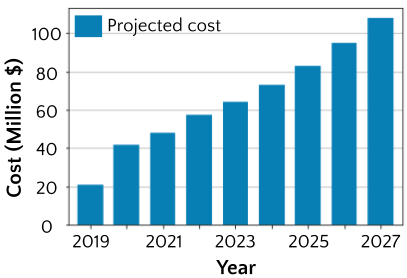
\includegraphics[height=3in]{include/project_costs_fig.png}
    \caption{\textbf{Projected cost of deploying finger pulse oximeters for telemedicine application.} HR sensing solutions for telemedicine and remote patient monitoring have relied on the adoption of wearable sensors. Currently, the most viable and inexpensive existing wearable solution to assess patient HR and oxygen saturation are finger pulse oximeters. For the scales at which telemedicine is projected to grow, such a solution would involve a deployment cost in excess of \$700 million in the US alone. In contrast, a smartphone camera-based method offers a purely algorithmic solution that can be integrated into existing healthcare system telemedicine video-conferencing applications.}
    \label{fig:projected_costs_pulseox}
\end{figure}

In contrast to wearable sensors, recent methods have proposed using camera-based hardware present on modern-day smartphones in combination with signal processing and computer vision algorithms to estimate key vital signs, including HR \cite{}. Given the high penetration of mobile phone technology globally \cite{}, such a solution would potentially have zero marginal cost, thereby offering clinicians a highly accessible and inexpensive method of assessing vital signs remotely. 

Camera-based HR sensing methods can be categorized into two distinct methodologies: contact-based and contactless. Contact-based methods, where the finger is typically placed overtop the camera module, have already seen widespread applications in major smartphones \cite{proesmans_mobile_2019,li_current_2019}. Such methods show good performance, however, their utility for telemedicine video-conferencing visits is potentially limited as the camera module is covered during measurement. This prevents continuous monitoring of patient HR, visual well-being, and collection of other vitals such as respiratory rate and spatial blood perfusion maps. Contactless methods circumvent this limitation by remotely extracting a blood volume pulse (BVP) signal and corresponding HR estimate traditionally from facial videos \cite{}. The consequence of capturing a larger field-of-view is a much weaker signal, and therefore worse performance. 

Remote photoplethysmography (r-PPG) is by far the most prominent technique used in literature for contactless camera-based HR sensing. R-PPG operates by looking for subtle color variations visible on the surface human skin, caused by sub-dermal light absorption fluctuations from changes in blood volume and content. Early work conducted by Verkruysse \textit{et al.} \cite{verkruysse_remote_2008} showed that plethysmographic signals could be measured using ambient light and a consumer-grade digital camera. In order to accurately isolate and extract the correct BVP signal corresponding to the HR, several r-PPG algorithms have been proposed, including blind source separation (BSS)~\cite{}, model-based~\cite{}, unsupervised data-driven~\cite{}, and supervised deep learning~\cite{} methods. Unfortunately, the performance of existing r-PPG algorithms fluctuates with changes in illumination condition (32), subject motion (19, 30, 33), and skin tone (40). Moreover, assessment of these algorithms has typically been done on computer vision datasets that are not focused on telemedicine applications. Consequently, these datasets do not represent characteristics that are important for clinical translation such as a large population with diverse skin tone and gender representation and video data collection on end-user devices such as smartphones. 

The focus of this thesis is on developing a contactless camera-based HR sensing method for smartphone deployment that can successfully translate to telemedicine application. In particular, this thesis specifically addresses the bias for skin tone present in r-PPG algorithms. We provide a theoretical framework to understand the unique physics that underlies the inconsistency in r-PPG measurement across skin tones. From this, we establish that the bias is due to imaging noise, and appropriately propose r-PPG denoising methods to alleviate performance losses, including a novel algorithm that achieves overall state-of-the-art performance and large performance gains for dark skin tones. To assess the performance of the proposed method, we collect the first remote vital signs detection dataset focused on telemedicine applications that is demographically diverse. 

\section{Contributions}

In context of prior r-PPG related works, this thesis demonstrates the following technical contributions:

\begin{enumerate}
    \item A light-transport theory for r-PPG application that provides novel mathematical insights of r-PPG performance and biases with respect to skin tone.
    \item The first clinical telemedicine-focused remote vital signs dataset, named VITAL, that contains a diverse population of subjects under a variety of recording conditions. 
    \item A novel r-PPG algorithm that achieves overall state-of-the-art performance and large performance gains for dark skin tones on the VITAL dataset.
\end{enumerate}

% \section{Organization}


  
%
% theory.tex
% Copyright (C) 2021 by Krish Kabra, <krish@kabra.com>.
%

\chapter{Theory}

\begin{figure}[t]
    \centering
    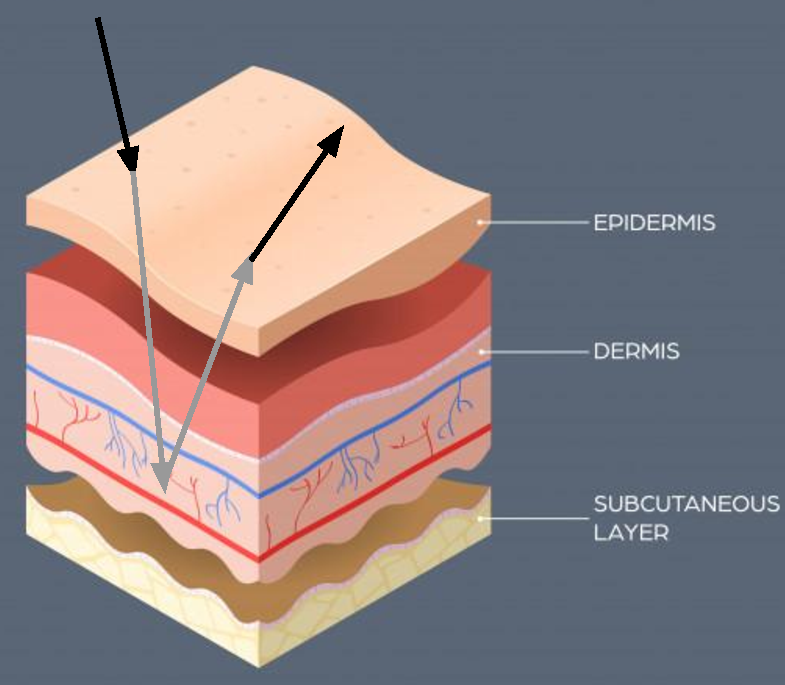
\includegraphics[height=3in]{include/fig_skin.pdf}
    \caption{\textbf{A two-layer skin model used in prior biorealistic rendering works is used to develop the light transport theory for R-PPG.} The incident light ray attenuates through the epidermis. Following dermal reflection and another epidermal attenuation, the resultant ray properties are dependent on human physiological quantities.}
    \label{fig:skin_model}
\end{figure}

Plethysmographic estimation methods are enabled through the sensing of blood perfusion in the face. Specifically, the presence of varying volumes of blood under the skin manifest as minute changes in reflection properties of the overall skin system, as viewed by a camera. It is by identifying these changes that relevant physiological properties may be estimated. 

In order to set up a novel light transport theory for R-PPG, we utilize existing biorealistic graphical rendering models~\cite{} and extend them for R-PPG signal generation. Figure~\ref{fig:skin_model} shows the skin model assumed for our computations, similar to~\cite{alotaibi_biophysical_2017}. Specifically, a two layer skin model is assumed. The incident light undergoes attenuation while passing through the epidermis, while it undergoes scattering driven reflection at the dermis. 

Using our light transport theory, we show that the signal strength reduces with increasing skin melanin content for all color channels, as intuitively expected. The decreasing signal strength leads us to an analysis of imaging noise, which is the major noise phenomenon at play in this case. Finally, with these mathematical insights, we conclude this section with a discussion on skin tone bias for r-PPG and propose solutions to improve performance on dark skin tone subjects.  

\section{Light Transport for R-PPG}

% \subsection{Epidermal Transmission}
We start with describing the epidermal transmission. Following the Beer-Lambert Law, 
\begin{equation} \label{eqn:T_epidermis}
    \mathbf{T_{epi}(\boldsymbol{\lambda})=e^{-\boldsymbol\mu_{a,epi}(\boldsymbol\lambda)}},
\end{equation}
Where $\mathbf{\boldsymbol\mu_{a,epi}(\boldsymbol\lambda)}$ is the absorption coefficient of the epidermis. Typically, this is modelled as a convex combination of skin tissue and melanin absorption,
\begin{equation} \label{eqn:mu_epidermis}
    \mathbf{\boldsymbol\mu_{a,epi}(\boldsymbol\lambda)=f_{mel}\boldsymbol\mu_{a,mel}(\boldsymbol\lambda)+(1-f_{mel})\boldsymbol\mu_{a,ski}(\boldsymbol\lambda)}.
\end{equation}

$\mathbf{\boldsymbol\mu_{a,ski}(\boldsymbol\lambda)}$, the skin tissue absorption coefficient, is a biological parameters which is known. $\mathbf{\boldsymbol\mu_{a,mel}(\boldsymbol\lambda)}$ may be defined as,
\begin{equation} \label{eqn:mu_melanin}
    \mathbf{\boldsymbol\mu_{a,mel}(\boldsymbol\lambda)=f_{eum}\boldsymbol\mu_{a,eum}(\boldsymbol\lambda)+(1-f_{eum})\boldsymbol\mu_{a,phm}(\boldsymbol\lambda)},
\end{equation}
Where ${\mathbf{\boldsymbol\mu_{a,eum}(\boldsymbol\lambda)}}$ is the absorption coefficient of eumelanin and $\mathbf{\boldsymbol\mu_{a,phm}(\boldsymbol\lambda)}$ is the absorption coefficient of pheomelanin, all biophysical known parameters. By combining Equations~\ref{eqn:T_epidermis}, \ref{eqn:mu_epidermis} and \ref{eqn:mu_melanin}, the epidermal transmission may be accurately modelled.

% \subsection{Dermal Reflection} 
We move towards describing the dermal reflection. This model follows the Kubelka-Munk theory for scattering-dependent reflection. Specifically, the fraction of reflected light, as a function of wavelength, is given by,
\begin{equation}
    \mathbf{R_{d}(\boldsymbol\lambda)=\frac{(1-\boldsymbol\beta(\boldsymbol\lambda))^2(e^{K(\boldsymbol\lambda)d_{der}}-e^{-K(\boldsymbol\lambda)d_{der}})}{(1+\boldsymbol\beta(\boldsymbol\lambda))^2e^{K(\boldsymbol\lambda)d_{der}}-(1-\boldsymbol\beta(\boldsymbol\lambda))^2e^{-K(\boldsymbol\lambda)d_{der}}}}
\end{equation}
Here, $\mathbf{\boldsymbol\beta(\boldsymbol\lambda)}$ and $\mathbf{K(\boldsymbol\lambda)}$ are deterministically related to $\mathbf{\boldsymbol\mu_{a,der}(\boldsymbol\lambda)}$ (dermal absorption coefficient) and $\mathbf{\boldsymbol\mu_{s,der}(\boldsymbol\lambda)}$ (reduced dermal scattering coefficient, known~\cite{}). Similar to previously, the dermal absorption coefficient and the blood absorption coefficient are understood as convex combinations shown below:
\begin{equation}
    \mathbf{\boldsymbol\mu_{a,der}(\boldsymbol\lambda)=f_{bld}\boldsymbol\mu_{a,bld}(\boldsymbol\lambda)+(1-f_{bld})\boldsymbol\mu_{a,ski}(\boldsymbol\lambda)}
\end{equation}
\begin{equation}
    \mathbf{\boldsymbol\mu_{a,bld}(\boldsymbol\lambda)=f_{oxy}\boldsymbol\mu_{oxy}(\boldsymbol\lambda)+(1-f_{oxy})\boldsymbol\mu_{dox}(\boldsymbol\lambda)}
\end{equation}
Here, various factors include blood reflection, skin baseline reflection, oxygenated blood reflection and deoxygenated blood reflection respectively.

% \subsection{Overall Reflection} 
Given the expressions for epidermal transmission and dermal reflection, the expression for overall reflection is given by,
\begin{equation}
    \mathbf{R(\boldsymbol\lambda) = T{^2}_{epi}.R_{d}(\boldsymbol\lambda)}.
\end{equation}

Then, the overall intensity captured in channel $\mathbf{c}$ of the camera is given by,
\begin{equation}
    \mathbf{I_c=\boldsymbol\int_{\boldsymbol\lambda}E(\boldsymbol\lambda)S_{c}(\boldsymbol\lambda)R(\boldsymbol\lambda)d\boldsymbol\lambda},
\end{equation}
Where $\mathbf{E(\boldsymbol\lambda)}$ is the source spectral distribution and $\mathbf{S_{c}(\boldsymbol\lambda)}$ is the camera spectral response for channel $\mathbf{c}$.

\section{R-PPG Signal Strength} 

\begin{figure}[t]
    \centering
    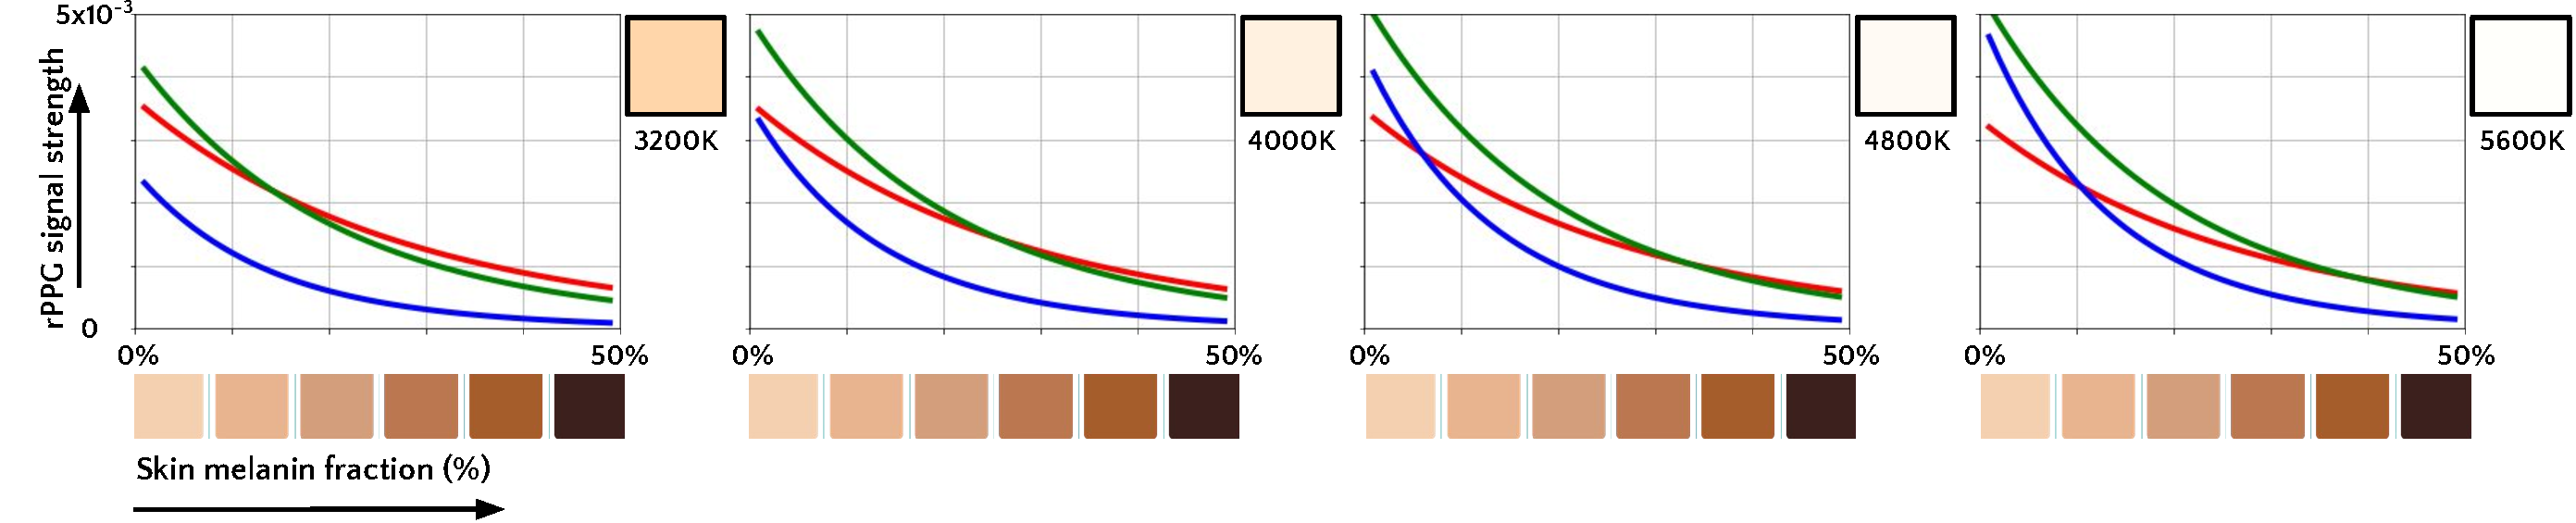
\includegraphics[width=\linewidth]{include/fig_strength.pdf}
    \caption{\textbf{The R-PPG signal strength is critically related to skin melanin fraction as well as scene lighting.} As opposed to previously accepted fact, the three channels may contain differing amounts of signal information, depending on regime of operation.}
    \label{fig:signal_strength}
\end{figure}

The R-PPG signal arises out of a variation in the blood volume fraction, $\mathbf{f_{bl}}$ under the skin. Our interest is in the signal strength across camera channels, $\boldsymbol\Sigma_{c}$, which can be defined as \textit{the maximum variation in the captured intensity}. Mathematically,
\begin{equation}
\begin{split}
    &\mathbf{\boldsymbol\Sigma_{c}=\boldsymbol\Delta I_c\boldsymbol\approx \Big|\frac{\boldsymbol\partial I_c}{\boldsymbol\partial f_{bl}}\Big|\cdot\boldsymbol\Delta f_{bl}}
\end{split}
\end{equation}
Since $\mathbf{R(\boldsymbol\lambda)}$ is the only term dependent on $\mathbf{f_{bl}}$,
\begin{equation}
\begin{split}
    &\mathbf{\boldsymbol\Sigma_{c}\boldsymbol\approx  \Big|\boldsymbol\int_{\boldsymbol\lambda}E(\boldsymbol\lambda)S_{c}(\boldsymbol\lambda)\frac{\boldsymbol\partial R}{\boldsymbol\partial f_{bl}}\Bigg|_{\overline{f_{bl}}} d\boldsymbol\lambda \Big| \cdot \boldsymbol\Delta f_{bl}},
\end{split}
\end{equation}
Where $\mathbf{\overline{f_{bl}}}$ is the average blood volume fraction, typically around $0.05$. This approximation holds true since $\mathbf{f_{bl}}$ only varies by a small amount, typically around $0.05$. 

This plethysmographic signal rides on top of the average skin tone color, given by
\begin{equation}
    \mathbf{\boldsymbol\Gamma_c=\boldsymbol\int_{\boldsymbol\lambda}E(\boldsymbol\lambda)S_{c}(\boldsymbol\lambda)R(\boldsymbol\lambda)\Big|_{\overline{f_{bl}}} d\boldsymbol\lambda}.
\end{equation}

Since, $\boldsymbol\Sigma_{c}$ and $\boldsymbol\Gamma_{c}$ are both dependent on $\mathbf{f_{mel}}$, as a result of the dependence of $\mathbf{R(\cdot)}$ on the same, we refer to these as $\mathbf{\boldsymbol\Sigma(f_{mel})}$ and $\mathbf{\boldsymbol\Gamma(f_{mel})}$ subsequently.

{\color{red} 
\begin{enumerate}
    \item Add parameter values used/the source paper for the same, for reproducability.
    \item Not clear what you mean by average camera response function. Also, where did we get the average response function from? We should cite our sources for reproducability. Same goes for light source characteristics.
\end{enumerate}
}

Figure~\ref{fig:signal_strength} shows the signal strength plots for the three camera color channels, across lighting conditions. We use average camera response functions $\mathbf{S_c(\boldsymbol\lambda)}$ to identify responsiveness of each of the channels to incident light. We also generate signal strength across common light source characteristics.  These plots provide incisive detail: the overall signal strength decays with increasing skin melanin fraction. Additionally, while previous works~\cite{verkruysse_remote_2008,haan_robust_2013,wang_algorithmic_2017} have empirically determined that the green channel holds maximum R-PPG signal information, we show for the first time that this in-fact heavily depends on melanin fraction. While the green channel is dominant for light skin tones, for darker skin tones, the channel-wise signal strength depends significantly on lighting conditions and skin tone.

\section{Effect of Imaging Noise on R-PPG}

\begin{figure}[t]
    \centering
    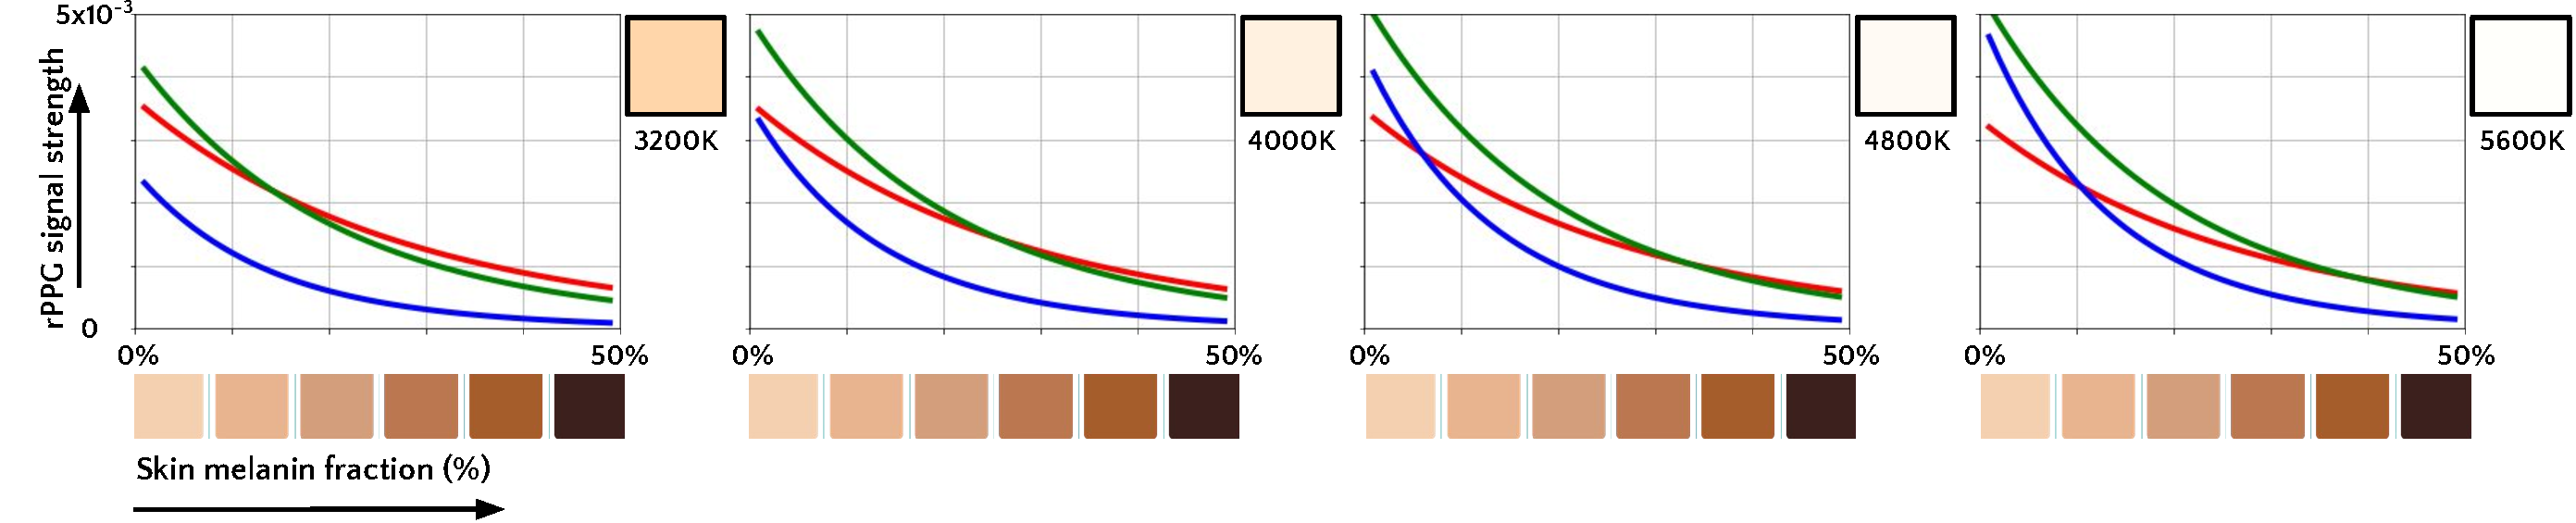
\includegraphics[width=\linewidth]{include/fig_strength.pdf}
    \caption{\textbf{FIGURE TO BE CHANGED!}}
    \label{fig:SNR_theory}
\end{figure}

The goal of this subsection is to understand the relationship between imaging noise and R-PPG algorithm estimation. Imaging noise refers to the inherent noise that arises due to the image capture process in a commercial camera. This arises due to various effects related to photon arrival processes, thermal noise in electronics and the quantization noise associated with digitally capturing images \cite{hasinoff_noise-optimal_2010}. For
pixels below the saturation level, the noise can be modelled as follows: 
\begin{equation} \label{eqn:imaging_noise_model}
    \sigma_{pixel}^2 = \frac{\Phi t}{g^2} + \frac{\sigma_{r}^2}{g^2} + \sigma_{q}^2
\end{equation}
where $\Phi$ is the radiant power of light collect, $t$ is the exposure time, $g$ is the sensor gain (a constant for a given image), and $\sigma_r$ and $\sigma_q$ are camera noie parameters (also constant). 

Using this noise model, we can the estimate the entire R-PPG signal to noise ratio (SNR) for a pixel of a particular intensity and color channel $c$ as follows:
\begin{equation} \label{eqn:SNR_rPPG}
    \mathbf{SNR_c} = \frac{\mathbf{\boldsymbol\Sigma_{c}}t}{\sqrt{\frac{\mathbf{\boldsymbol\Gamma_{c}}t}{g^2} + \frac{\sigma_{r}^2}{g^2} + \sigma_{q}^2}}
\end{equation}
Here, we assume that the radiant power of light collected $\Phi$ is equal to the average skin tone color. 

Figure~\ref{fig:SNR_theory} shows... These observations leads us to inferences

\section{Origins of Skin Tone Bias}

In recent years, the task

\cite{kadambi_achieving_2021}


\begin{enumerate}
    \item \textit{Imaging noise creates skin tone bias (and lighting bias)}

\end{enumerate}

\begin{figure}[t]
    \centering
    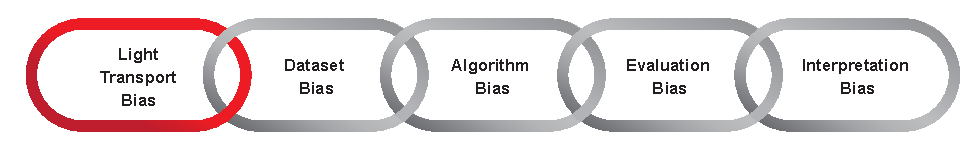
\includegraphics[width=\linewidth]{include/F_chain2.pdf}
    \caption{\textbf{The chain of biases in vision.}}
    \label{fig:chain_bias}
\end{figure}


% In recent years, there has been increasing interest in promoting the fairness of computer vision systems. A biased vision system for a task T, may operate differently when applied to certain subgroups of people or objects. To address this complex issue of fairness, colleagues have rightly pointed out factors that include dataset bias, algorithmic bias, or decision-making bias. However, there is another type of bias that is less discussed: the bias encountered by the laws of physics. Computer vision relies on light-sensing cameras - what if the physics of light involves bias? As one example, consider the task of face recognition with color cameras. We can immediately observe that a light-skinned face will fundamentally reflect more light (i.e. signal) than a dark-skinned face. More nuanced, however, are factors like the oiliness and texture of the face, which vary between males and females. These are forms of low-level bias. In this proposal, the PI lays the foundation for studying physical bias in a principled manner motivated by physics-based theory, experimental simulations, and ultimately the design of a novel colorless computational camera and health imagers that work consistently across skin tones. The work builds upon the PI’s deep expertise in low-level vision, imaging physics, and computational imaging. Further, the work lays a foundation for bringing physics into the realm of fair computer vision. 



% \section{Bias in R-PPG}

% \subsection{Algorithm Bias}

% \subsection{Dataset Bias}

% \subsection{Light Transport Bias}

  
%
% methods.tex
% Copyright (C) 2021 by Krish Kabra, <krish@kabra.com>.
%

\chapter{Methods}

\textbf{Overview of methods section...}

\section{VITAL Dataset}

\begin{figure}
    \centering
    \includegraphics[width=\linewidth]{include/exp_setup.pdf}
    \caption{\textbf{Constructing a diverse remote vital sign monitoring dataset with a focus on telemedicine applications.} (a) Cartoon schematic depicting the telemedicine application for the proposed camera-based heart rate estimation. (b) Telemedicine video-conferencing applications can be integrated with a software toolkit to display patient BVP and HR. (c) Experimental setup employed during the construction of the VITAL dataset. Two bi-color LEDs are used for controlled illumination of the subject, and laboratory tube LEDs are used for ambient illumination. The Philips IntelliVue MX800 patient monitor is utilized for ground truth vital sign monitoring. Two smartphone cameras at differing viewing angles capture video of the subject. (d) Example frame from video captured by the smartphone camera. The subject wears a blood pressure cuff, 5-ECG leads, and a finger pulse oximeter, which is connected to the MX800 unit. Written consent was obtained from the subject for using their image in the publication.}
    \label{fig:exp_setup}
\end{figure}

To validate the performance of camera-based vital sign detectors, we construct the Vital-sign Imaging for Telemedicine AppLications (VITAL) dataset. The focus of this dataset is to represent diversity in factors that are relevant to telemedicine setups, including: (i) smartphone deployment, (ii) camera view angle, (iii) recording condition (lighting variation and talking), and (iv) patient demographic diversity. We address each of these aspects individually:

\begin{enumerate}[label=(\roman*)]
    \item \textbf{Smartphone deployment:} The ubiquity of smartphones globally has led to the development of patient portals, many of which can be accessed via smartphone applications that can be downloaded by patients (45–47). Such applications have been used for hosting telemedicine appointments. A deployable remote HR estimation solution with a focus on telemedicine must be able to work efficiently on smartphone cameras by considering factors including video compression (23, 42, 48) and algorithmic complexity. Moreover, the solution must achieve success independent of camera type. Hence, the VITAL dataset uses different smartphone cameras for each view angle. The use of more than one smartphone imager inspires the development of algorithms that can scale to a variety of device-agnostic telemedicine conditions. 
    \item \textbf{Camera view angle:} In a telemedicine setting, there can also be a variety of camera angles that the algorithm must work on. In order to facilitate this verification, the VITAL dataset consists of two camera view angles for all the videos of each subject (as seen in Figure~\ref{fig:exp_setup}).
    \item \textbf{Recording condition:} Another essential factor involves testing algorithms across a range of recording conditions, to promote the development of algorithms that can operate in the “wild”. The dataset consists of four recording conditions: (1) controlled lighting at 5600K (“cool” lighting) with the subject remaining stationary, (2) controlled lighting at 3200K (“warm” lighting) with the subject remaining stationary, (3) ambient room lighting- distributed white lighting- with the subject remaining stationary, and (4) ambient room lighting with the subject speaking. Additionally, a green screen backdrop is kept to potentially enable digital modification of background scenery.
    \item \textbf{Patient demographic diversity:} The VITAL dataset consists of 54 subjects spread across skin tone, age, gender, race, and ethnic backgrounds. Subject characteristics (gender, age, height, weight, body mass index, race, and ethnicity) are summarized in Table 1 using mean (SD), median (IQR), or frequency (\%), unless otherwise noted. For the purpose of this study, we split the subjects into three skin tone categories based on the Fitzpatrick (FP) skin type scale (49): light, consisting of skin tones in the FP 1 and 2 scales, medium, consisting of skin tones in the FP 3 and 4 scales, and dark, consisting of skin tones in the FP 5 and 6 scales. This aggregation allows for more relevant trends, since any two consecutive FP scale categories are reasonably close.
\end{enumerate}

The human study protocol was approved by the UCLA Institutional Review Board (IRB\#20-001025-AM-00001), and participants provided written informed consent to take part in the study. Figure~\ref{fig:exp_setup} shows the data collection setup. Each subject is made to sit on a height-adjustable chair, in the field of view of two cell-phone cameras (with different view angles): one camera (Samsung Galaxy S10) is perfectly front-on, while the other (Samsung Galaxy A51) is directly in front of the face, at a dip (lower) of 15 degrees. The front-on camera is placed approximately 130 cm from the subject, and the lower camera at a dip is approximately 90 cm from the subject. The height of the chair is chosen so that the subject is centered in the front-on frame. The controlled lights are set up on either side of the front-on camera, with a baseline of 100 centimeters between them.

As aforementioned, we record subjects using these cameras under four different scene conditions: (1) controlled lighting at 5600K (“cool” lighting) with the subject remaining stationary, (2) controlled lighting at 3200K (“warm” lighting) with the subject remaining stationary, (3) ambient room lighting (distributed white LED lighting) with the subject remaining stationary, and (4) ambient room lighting with the subject speaking. Controlled lighting is enabled by a pair of professional bi-color LED photography lights (Neewer Bi-Color 480 LED). The controlled lighting recording conditions were enabled with the room lights off, allowing for fine-tuned control over the illumination spectral properties. As incorporating controlled lighting only enables a front-facing illumination angle, two recording conditions in ambient room lighting were captured where the subject was lit more completely from several angles. The final recording condition involved variations in the subject, including talking, natural head movements, and facial expressions. Each scene recording session lasts for 2 minutes, for a total of 16 minutes of video footage across 8 videos. 

During data collection, volunteers are fitted with standard anesthesiology cardiopulmonary monitors: pulse oximeter (Red DCI, Masimo), blood pressure cuff (Comfort Care, Philips), and 5-lead electrocardiogram (Philips IntelliVue). To collect vital sign data, we utilize the Philips IntelliVue MX800 patient monitor to perform real time monitoring of four vital signs- HR, respiratory rate, oxygen saturation, and non-invasive continuous blood pressure- of which three waveforms are collected (ECG, PPG and respiration). We use the open source tool VSCapture (61) to collect data onto a computer using the MX800’s local area network communication protocol. The MX800’s estimated numeric values for the vital signs are sampled every 1 second, while the waveforms are sampled at variable frequencies. The ECG signal is sampled between 400-600 Hz, the PPG signal between 100-150Hz and the respiration between 40-60Hz.  Continuous non-invasive blood pressure estimates occur when the blood pressure cuff is activated, which is approximately once every 30 seconds. 

\section{Algorithmic principles of R-PPG}

\section{Denoising strategies}

\section{Diverse R-PPG}

  
%
% results.tex
% Copyright (C) 2021 by Krish Kabra, <krish@kabra.com>.
%

\chapter{Results}

\section{Statistical analysis}

\section{Overall performance}

\section{Skin tone performance}

\section{Recording condition performance}

\section{Camera viewpoint performance}

  
%
% conclusions.tex
% Copyright (C) 2021 by Krish Kabra, <krish@kabra.com>.
%

\chapter{Conclusions} \label{chap:conclusion}

In this thesis, we propose a novel R-PPG algorithm to estimate subject HR in a contactless manner using only a smartphone camera. Several R-PPG algorithms have been proposed to extract the BVP signal from videos; however, these algorithms exhibit a performance gap, and therefore a bias, for certain types of skin tones \cite{nowara_meta-analysis_2020}, subject motions (e.g. speaking) \cite{mocco_motion_2016,de_haan_improved_2014,wang_exploiting_2015}, and illumination conditions \cite{li_remote_2014}. Addressing these biases is essential for successful deployment of R-PPG technology in telemedicine applications, yet it remains a challenge. For example, we mathemetically show that dark skin, which contains higher amounts of melanin, fundamentally reduces the SNR of  R-PPG. Nowara et al. \cite{nowara_meta-analysis_2020} highlights this reduction, thereby conclusively determining that current R-PPG algorithms have markedly worse performance on darker skin tones. The work also highlights the issue of biased skin tone and gender representation in computer vision datasets, which is especially true for the comparatively small datasets used in R-PPG analyses. This dataset bias further prevents underlying light-transport biases, such as skin tone bias, from being addressed. Should contactless HR sensing using video be implemented in a clinical setting, the development of R-PPG computer vision algorithms and datasets that improve the accuracy and reduce the bias of HR measurements for patients of all skin tones (especially the darker skin tones) is critically necessary for high-quality telemedicine care.

A key contribution of this work is the creation of the VITAL dataset, which is a first effort towards collecting a demographically diverse video vital sign database for telemedicine applications. While societal demographics are skewed largely towards light skin tone persons, it is essential to have diversely represented computer vision healthcare datasets to understand performance limitations that may otherwise be masked within biased data \cite{cahan_putting_2019}. Although the VITAL dataset is not entirely unbiased itself, it achieves a much higher degree of skin tone diversity as compared to existing datasets. Moreover, the VITAL dataset records facial videos using smartphone cameras, which introduces significant video compression and imaging noise artifacts. Typically, R-PPG methods are developed and tested using uncompressed videos. However, deployment of R-PPG technology for telemedicine will ultimately require a robustness to video compression noise artifacts. Therefore, the VITAL dataset enables a more realistic evaluation of remote video-based vital sign monitoring methods for telemedicine translation, which contrasts from previous works. Finally, the VITAL dataset captures four ground truth vital signs: HR, respiratory rate, oxygen saturation, and non-invasive continuous blood pressure, of which three waveforms are collected: ECG, PPG and respiration. Although this work only utilizes the HR obtained from the PPG waveform for testing, we anticipate future work capturing all four vital signs simultaneously from the facial videos. Overall, we envision the VITAL dataset to be an essential resource for upcoming related research and, in addition, to set the tone for future data collection endeavors for similar interdisciplinary clinical cum technological applications.

With respect to algorithmic development, this work addresses the aforementioned biases in skin-tone, illumination conditions, and subject motions using physics-rooted knowledge and camera noise analysis. From our theory, we derive 2 key conclusions: (i) imaging noise creates skin tone bias (and lighting bias), and (ii) imaging noise and specular reflections degrade the R-PPG signal. Therefore, we primarily focus our attention to signal processing strategies as opposed to signal extraction modifications. The first attempted work to reduce R-PPG skin tone bias was done by Kumar et al. (DistancePPG) \cite{kumar_distanceppg_2015}, in which a weighted average of BVP signals from various facial ROIs. However, to the best of the authors’ knowledge, no work yet has continued development of R-PPG algorithms that tackle the important issue of performance bias on darker skin tones. The proposed R-PPG algorithm draws from existing R-PPG denoising methods that use a similar weighted ROI philosophy as in DistancePPG (c.f. \cite{po_block-based_2018,li_model-based_2020,bobbia_unsupervised_2019}). Specifically, it modifies the signal combination step by combining signal information from various facial ROIs in the frequency-domain rather than the time-domain. Moreover, it introduces a skin diffuse component weighting when averaging the signal information. This enables the proposed algorithm to drastically mitigate performance losses for subjects with darker skin tones, subjects in varying illumination conditions, and subjects who may be moving their face such as when they are talking. 

The proposed method achieves the best overall average MAE performance across the VITAL dataset of 7.62 bpm, as opposed to 10.04 bpm by the facial aggregation method \cite{poh_noncontact_2010,haan_robust_2013,wang_novel_2016,wang_algorithmic_2017,lewandowska_measuring_2011,de_haan_improved_2014} and 10.48 bpm for the SNR weighting method \cite{po_block-based_2018,li_model-based_2020,kumar_distanceppg_2015,bobbia_unsupervised_2019}. This achievement can be attributed to the performance gains seen across all skin tones in comparison to the facial aggregation method. The SNR weighting method shows performance gain only for the light skin tone subjects (+0.39 bpm) and a performance drop for the medium and dark skin tones (-1.22 and -0.24 bpm respectively), thereby actually increasing the skin tone performance bias. Consequently, the method’s overall performance suffers on a more diversely represented dataset such as VITAL. This illustrates the importance for the need of a truly diverse dataset when developing R-PPG technology.

Nevertheless, as with previous methods, the performance of the proposed method still exhibits a skin-tone bias. However, we highlight that the proposed method achieves the largest MAE improvements over the facial aggregation method of 28.5\% (+4.11 bpm) for the traditionally worse performing dark skin tone in comparison with the light (20.2\%, +1.71 bpm) and medium (23.7\%, +2.22 bpm) skin tones. This outcome attests to the fairness of the method. The proposed method is the only method able to perform with an overall MAE less than 8 bpm across all skin tones. These inferences are further enforced by the significant decrease in the SDE and overall improvement in the correlation coefficient, as opposed to the SNR weighting method which sees performance reduction for medium and dark skin tones. Hence, in addition to the overall improvement in performance across all skin tones, the proposed method successfully steps towards reducing the performance bias that exists between skin tones. If the VITAL dataset were to have even more equal representation in terms of skin tone, the overall average performance measures are further expected to improve. 

Large improvements in performance of the proposed method are also observed for the talking activity over the facial aggregation benchmark, as compared to the SNR weighting method which shows an overall performance drop. This technology may one day allow for real-time continuous contact-less HR monitoring during a telemedicine visit, which would provide greater information to outpatient clinicians. This advance may also be relevant for in-hospital continuous contactless monitoring in ICU settings or hospital floor care.
Improvements in performance are also observed across camera viewpoints. The proposed method shows considerable improvements for the front and bottom angles. A typical telemedicine visit, through a cell phone platform, may involve the patient holding the camera at varying angles with respect to the face. The shown robustness and performance improvement of the proposed method therefore makes it increasingly amenable to such tasks. Interestingly, for all methods tested (existing and novel), the bottom angle shows improved performance as compared to the front angle. This could be because interfering factors such as hair, spectacles and so on occupy a smaller portion of the usable frame in the bottom angle, as well as differing face scales in the two angles.

In relation to the clinical significance of this work, remote vital sign monitoring has risen in prominence over recent years, with an acceleration in clinical development due to the COVID-19 pandemic. In response to the pandemic, health systems across the country implemented a large-scale restriction of non-urgent in-person appointments \cite{jm_virtual_2020}, transitioned many outpatient services to telemedicine visits \cite{connolly_rapid_2020}, and developed remote monitoring care pathways \cite{annis_rapid_2020} in order to facilitate social distancing yet maintain continuity of care. To remotely monitor COVID-19 patients, many health systems shipped home vital sign equipment to patients in order to obtain quantitative physiological data that could facilitate high quality remote management via telemedicine. At a population level, however, supplying and shipping vital sign monitoring devices to patients is expensive and not scalable, making such a solution nonviable. For the scales at which telemedicine is projected to grow, the projected cost of deploying finger pulse oximeters for telemedicine application, the most viable and inexpensive existing solution to assess patient HR and oxygen saturation, would involve a deployment cost in excess of \$700 million in the US alone (see Appendix~\ref{chap:telemedicine_cost_projections} for calculation details) \cite{polaris_us_2020}. Given the high penetration of mobile phone technology globally \cite{pew_demographics_2019}, there is great interest in transforming smartphones into low-cost portable HR, respiratory rate, and pulse oximeter monitors, thereby increasing accessibility to vital monitoring equipment and alleviating healthcare inequity. Using in-built camera modules and computer vision algorithms to obtain quantitative vital sign data remotely offers a purely algorithmic solution with potentially zero marginal cost. 

Outside of a pandemic situation, knowledge of vital signs is also important information for clinicians who are managing medical conditions that require such data for health management, and remotely obtaining vital signs may allow care teams to perform remote surveillance and home monitoring of patients with greater confidence. Notably, several minority and lower socioeconomic status patient populations may benefit from more remote care, especially as it has been established that the COVID-19 pandemic has disproportionately affected such communities, both nationally and in states the most affected by the pandemic \cite{abedi_racial_2020,azar_disparities_2020}. In New York City and Michigan, African American and Latino residents have the highest age-adjusted rates of hospitalized and non-hospitalized COVID-19, and age-adjusted death rates for African Americans are more than twice those for white and Asian residents \cite{holtgrave_assessing_2020,gu_characteristics_2020}. African American communities have also been found to have higher prevalence of cardiovascular and related complications, when compared with traditionally light skin toned people \cite{mensah_cardiovascular_2018}. These patient populations may therefore stand to benefit the most from skin tone robust contactless vital sign (specifically heart rate) sensing technologies that facilitate high-quality remote care pathways. Finally, we believe contactless vital sign sensing technology would be useful at the start of in-person clinic or hospital encounters or for continuous patient monitoring in a hospital floor or ICU setting. Cameras, as opposed to hospital staff, may one day obtain key vital signs without contact, thereby reducing exposure of patients to staff, enabling improved infection control, and freeing up hospital staff to attend to other important patient care needs.  

With regards to limitations and future work, while our method has been tested on an adult population, additional work is needed to enable clinical adoption.  Further research investigating HR estimation using our proposed method is still needed in pediatric and geriatric populations and patient populations with known cardiopulmonary disease. Future work must also focus on improving computer vision methods to detect extremes of HR and discern heart arrhythmias. Additionally, the proposed method does not obviate skin tone bias but rather is the first work that can be demonstrated to mitigate skin tone bias in the VITAL dataset. Therefore, research must be undertaken to further reduce bias and assure fairness by building upon our work, as well as to continue improving overall performance on subjects and videos in real life scenarios. 
 
From an algorithmic perspective, we believe that one of the most important factors towards large scale deployment of such methods for clinical use is the inherent fairness of the algorithm. As healthcare increasingly accelerates towards a digitally connected and virtual future, early consideration must be given to developing equitable health technology that does not exacerbate healthcare disparities or create new disparities. Ultimately, we hope this work motivates the community towards exciting and essential research avenues looking into inherent system biases associated with R-PPG. By reducing biases, we move a step closer towards deploying high-quality, medically inclusive non-contact vital sensing techniques that can aid clinicians in delivering remote patient care, during times of peace and pandemic alike.



  
\appendix
%
% appendix.tex
% Copyright (C) 2021 by Krish Kabra, <krish@kabra.com>.
%

\chapter{Deployment Cost Projections for Telemedicine}
\label{chap:telemedicine_cost_projections}

In order to calculate the estimated average deployment cost for the cheapest existing method (finger pulse oximeters), we use the following methodology:
\begin{enumerate}
    \item We identify the estimated user base numbers for telemedicine in the US using the numbers from \cite{kats_us_2020} and extend these up to 2027 using the compound annual growth rate (CAGR) of 15.8\% as suggested in \cite{polaris_us_2020}.
    
    \item We make the conservative assumption that all members of a given family would be active users of telemedicine services. Therefore, an estimate of the number of families using telemedicine services is given by: 
    \begin{equation}
        No.~of~Families = \frac{Number~of~Telemedicine~Users}{Avg.~Family~Size~in~the~US}
    \end{equation}
    We use the average family size of 3.15 from the U.S. Census Bureau's Current Population Survey \cite{cps_us_2020}.
    
    \item Assuming that one pulse oximeter costs \$20 (as observed from a survey of available units in the market), and assuming conservatively that one pulse oximeter has to be deployed per family, the cost of deployment is given by: 
    \begin{equation}
        Cost~of~Deployment = No.~of~Families~\times~Cost~per~Pulse~Oximeter~Unit
    \end{equation}
\end{enumerate}







  

\bibliographystyle{IEEEtran}
\bibliography{references}    % bibliography references

\end {document}